\chapter{Void methods}
\label{chap03}

\section{Floating-point}
\index{floating-point}
\index{type!double}
\index{double(floating-point)}

In the last chapter we had some problems dealing with numbers
that were not integers.  We worked around the problem by measuring
percentages instead of fractions, but a more general solution is
to use floating-point numbers, which can represent fractions
as well as integers.  In Java, the floating-point type is
called {\tt double}, which is short for ``double-precision.''

You can create floating-point variables and assign values to them
using the same syntax we used for the other types.  For example:

\begin{code}
    double pi;
    pi = 3.14159;
\end{code}
%
It is also legal to declare a variable and assign a value to it at the
same time:

\begin{code}
    int x = 1;
    String empty = "";
    double pi = 3.14159;
\end{code}
%
This syntax is common; a combined declaration
and assignment is sometimes called an {\bf initialization}.
\index{initialization}

Although floating-point numbers are useful, they are
a source of confusion because there seems to be an
overlap between integers and floating-point numbers.  For
example, if you have the value {\tt 1}, is that an integer,
a floating-point number, or both?

Java distinguishes the integer value {\tt 1}
from the floating-point value {\tt 1.0}, even though they
seem to be the same number.  They belong to
different types, and strictly speaking, you are not allowed
to make assignments between types.  For example, the following
is illegal:

\begin{code}
    int x = 1.1;
\end{code}
%
because the variable on the left is an {\tt int}
and the value on the right is a {\tt double}.  But it is easy
to forget this rule, especially because there are places where Java
will automatically convert from one type to another.
For example:

\begin{code}
    double y = 1;
\end{code}
%
should technically not be legal, but Java allows it by converting the
{\tt int} to a {\tt double} automatically.  This leniency is
convenient, but it can cause problems; for example:

\begin{code}
    double y = 1 / 3;
\end{code}
%
You might expect the variable {\tt y} to get the value
{\tt 0.333333}, which is a legal floating-point value, but in
fact it gets {\tt 0.0}.  The reason is that the
expression on the right is the ratio of two integers,
so Java does {\em integer} division, which yields the integer
value {\tt 0}.  Converted to floating-point, the result is
{\tt 0.0}.

One way to solve this problem (once you figure out what
it is) is to make the right-hand side a floating-point
expression:

\begin{code}
    double y = 1.0 / 3.0;
\end{code}
%
This sets {\tt y} to {\tt 0.333333}, as expected.

\index{arithmetic!floating-point}

The operations we have seen so far---addition, subtraction,
multiplication, and division---also work on floating-point values,
although you might be interested to know that the underlying mechanism
is completely different.  In fact, most processors have special
hardware just for performing floating-point operations.


\section{Converting from {\tt double} to {\tt int}}
\label{rounding}
\index{rounding}
\index{typecasting}

As I mentioned, Java converts {\tt int}s
to {\tt double}s automatically if necessary, because no
information is lost in the translation.  On the other hand,
going from a {\tt double} to an {\tt int} requires rounding
off.  Java doesn't perform this operation automatically, in
order to make sure that you, as the programmer, are aware
of the loss of the fractional part of the number.

The simplest way to convert a floating-point value to an integer is to
use a {\bf typecast}.  Typecasting is so called because it allows you
to take a value that belongs to one type and ``cast'' it into another
type (in the sense of molding or reforming).

The syntax for typecasting is to put
the name of the type in parentheses and use it as an operator.
For example,

\begin{code}
    double pi = 3.14159;
    int x = (int) pi;
\end{code}
%
The {\tt(int)} operator has the effect of converting what
follows into an integer, so {\tt x} gets the value 3.

Typecasting takes precedence over arithmetic operations,
so in the following example, the value of {\tt pi} gets
converted to an integer first, and the result
is 60.0, not 62.

\begin{code}
    double pi = 3.14159;
    double x = (int) pi * 20.0;
\end{code}
%
Converting to an integer always rounds down, even if the fraction
part is 0.99999999.  These behaviors (precedence and rounding)
can make typecasting error-prone.


\section{Math methods}
\index{Math class}
\index{class!Math}
\index{expression}
\index{argument}

In mathematics, you have probably seen functions like $\sin$ and
$\log$, and you have learned to evaluate expressions like
$\sin(\pi/2)$ and $\log(1/x)$.  First, you evaluate the
expression in parentheses, which is called the {\bf argument} of the
function.
Then you can evaluate the function itself, either by looking it up in
a table or by performing various computations.

This process can be applied repeatedly to evaluate more complicated
expressions like $\log(1/\sin(\pi/2))$.  First we evaluate the
argument of the innermost function, then evaluate the function,
and so on.

Java provides functions that perform the most
common mathematical operations.  These functions
are called {\bf methods}.
The math methods are invoked using a syntax that is similar to
the {\tt print} statements we have already seen:

\begin{code}
     double root = Math.sqrt(17.0);
     double angle = 1.5;
     double height = Math.sin(angle);
\end{code}
%
The first example sets {\tt root} to the square root of 17.
The second example finds the sine of the value of {\tt angle},
which is {\tt 1.5}.  Java assumes that the
values you use with {\tt sin} and the other trigonometric functions
({\tt cos}, {\tt tan}) are in {\em radians}.  To
convert from degrees to radians, you can divide by 360
and multiply by $2 \pi$.  Conveniently, Java provides {\tt Math.PI}:

\begin{code}
     double degrees = 90;
     double angle = degrees * 2 * Math.PI / 360.0;
\end{code}
%
Notice that {\tt PI} is in all capital letters.  Java does
not recognize {\tt Pi}, {\tt pi}, or {\tt pie}.

Another useful method in the {\tt Math} class is {\tt round},
which rounds a floating-point value off to the nearest integer
and returns an {\tt int}.

\begin{code}
    int x = Math.round(Math.PI * 20.0);
\end{code}
%
In this case the multiplication happens first, before the
method is invoked.  The result is 63 (rounded up from 62.8319).


\section {Composition}
\label{composition}
\index{composition}
\index{expression}

Just as with mathematical functions, Java methods can be {\bf
composed}, meaning that you use one expression as part of another.
For example, you can use any expression as an argument to a method:

\begin{code}
    double x = Math.cos(angle + Math.PI/2);
\end{code}
%
This statement takes the value {\tt Math.PI}, divides it by two and
adds the result to the value of the variable {\tt angle}.  The sum is
then passed as an argument to {\tt cos}. ({\tt
PI} is the name of a variable, not a method, so there are no
arguments, not even the empty argument {\tt()}).

You can also take the result of one method and pass it as
an argument to another:

\begin{code}
    double x = Math.exp(Math.log(10.0));
\end{code}
%
In Java, the {\tt log} method always uses base $e$, so this
statement finds the log base $e$ of 10 and then raises $e$ to that
power.  The result gets assigned to {\tt x}; I hope you know what it
is.

\section{Adding new methods}
\label{adding_methods}
\index{method!definition}
\index{main}
\index{method!main}

So far we have used methods from Java libraries,
but it is also possible to add new methods.  We have already
seen one method definition: {\tt main}.  The method named {\tt main}
is special, but the syntax is the same for other methods:

\begin{code}
  public static void NAME( LIST OF PARAMETERS ) {
    STATEMENTS
  }
\end{code}
%
You can make up any name you want for your method, except
that you can't call it {\tt main} or any
Java keyword.  By convention, Java methods start with a lower
case letter and use ``camel caps,'' which is a cute name for
{\tt jammingWordsTogetherLikeThis}.

The list of parameters specifies what information, if any, you have to
provide to use (or {\bf invoke}) the new method.

The parameter for {\tt main} is {\tt String[] args}, which
means that whoever invokes {\tt main} has to provide an array of
Strings (we'll get to arrays in Chapter~\ref{arrays}).  The first
couple of methods we are going to write have no parameters, so the
syntax looks like this:

\begin{code}
  public static void newLine() {
    System.out.println("");
  }
\end{code}
%
This method is named {\tt newLine}, and the empty parentheses
mean that it takes no parameters.  It contains one
statement, which prints an empty {\tt String}, indicated by {\tt ""}.
Printing a {\tt String} with no letters in it may not seem all that
useful, but {\tt println} skips to the next
line after it prints, so this statement skips to the next line.

In {\tt main} we invoke this new method the same way we invoke
Java methods:

\begin{code}
  public static void main(String[] args) {
    System.out.println("First line.");
    newLine();
    System.out.println("Second line.");
  }
\end{code}
%
The output of this program is

\begin{minipage}{\linewidth}
\begin{stdout}
First line.

Second line.
\end{stdout}
\end{minipage}

Notice the extra space between the lines.  What if we wanted
more space between the lines?  We could invoke the same
method repeatedly:

\begin{code}
  public static void main(String[] args) {
    System.out.println("First line.");
    newLine();
    newLine();
    newLine();
    System.out.println("Second line.");
  }
\end{code}
%
Or we could write a new method, named {\tt threeLine}, that
prints three new lines:

\begin{code}
  public static void threeLine() {
    newLine();  newLine();  newLine();
  }

  public static void main(String[] args) {
    System.out.println("First line.");
    threeLine();
    System.out.println("Second line.");
  }
\end{code}
%
You should notice a few things about this program:

\begin{itemize}

\item You can invoke the same procedure more than once.

\item You can have one method invoke another method.  In this
case, {\tt main} invokes {\tt threeLine} and {\tt threeLine}
invokes {\tt newLine}.

\item In {\tt threeLine} I wrote three statements all on the same
  line, which is syntactically legal (remember that spaces and new
  lines usually don't change the meaning of a program).  It is usually
  a good idea to put each statement on its own line, but I sometimes
  break that rule.

\end{itemize}

You might wonder why it is worth the trouble to
create all these new methods.  There are several
reasons; this example demonstrates two:

\begin{enumerate}

\item Creating a new method gives you an opportunity to
give a name to a group of statements.  Methods can simplify a program
by hiding a complex computation behind a single statement, and by using
English words in place of arcane code.  Which is clearer, {\tt
newLine} or {\tt System.out.println("")}?

\item Creating a new method can make a program smaller by eliminating
repetitive code.  For example, to print nine consecutive
new lines, you could invoke {\tt threeLine} three times.

\end{enumerate}

In Section~\ref{methods} we will come back to this question and list
some additional benefits of dividing programs into methods.


\section{Classes and methods}
\index{class}
\index{method}

Pulling together the code fragments from the previous
section, the class definition looks like this:

\begin{code}
class NewLine {

  public static void newLine() {
    System.out.println("");
  }

  public static void threeLine() {
    newLine();  newLine();  newLine();
  }

  public static void main(String[] args) {
    System.out.println("First line.");
    threeLine();
    System.out.println("Second line.");
  }
}
\end{code}
%
The first line indicates that this is the class definition for a new
class called {\tt NewLine}.  A {\bf class} is a collection of related
methods.  In this case, the class named {\tt NewLine} contains three
methods, named {\tt newLine}, {\tt threeLine}, and {\tt main}.

The other class we've seen is the {\tt Math} class.  It contains
methods named {\tt sqrt}, {\tt sin}, and others.  When
we invoke a mathematical method, we have to specify
the name of the class ({\tt Math}) and the name of the method.
That's why the syntax is slightly different for Java
methods and the methods we write:

\begin{code}
    Math.pow(2.0, 10.0);
    newLine();
\end{code}
%
The first statement invokes the {\tt pow} method in
the {\tt Math class} (which raises the first argument to the
power of the second argument).  The second statement invokes
the {\tt newLine} method, which Java assumes is in the class
we are writing (i.e., {\tt NewLine}).

If you try to invoke a method from the wrong class, the
compiler will generate an error.  For example, if you
type:

\begin{code}
    pow(2.0, 10.0);
\end{code}
%
The compiler will say something like, ``Can't find a method
named {\tt pow} in class {\tt NewLine}.''  If you have
seen this message, you might have wondered why it was looking
for {\tt pow} in your class definition.  Now you know.


\section {Programs with multiple methods}

When you look at a class definition that contains several methods, it
is tempting to read it from top to bottom, but that is likely to be
confusing, because that is not the {\bf order of execution} of the
program.

Execution always begins at the first statement of {\tt main},
regardless of where it is in the program (in this example I deliberately
put it at the bottom).  Statements are executed one at a time, in
order, until you reach a method invocation.  Method invocations are
like a detour in the flow of execution.  Instead of going to the next
statement, you go to the first line of the invoked method, execute all
the statements there, and then come back and pick up again where you
left off.

That sounds simple enough, except that you have to remember that one
method can invoke another.  Thus, while we are in the middle of {\tt
main}, we might have to go off and execute the statements in {\tt
threeLine}.  But while we are executing {\tt threeLine}, we get
interrupted three times to go off and execute {\tt newLine}.

For its part, {\tt newLine} invokes
{\tt println}, which causes yet another detour.  Fortunately,
Java is adept at keeping track of where it is, so when
{\tt println} completes, it picks up where it left off in
{\tt newLine}, and then gets back to {\tt threeLine}, and then
finally gets back to {\tt main} so the program can terminate.

Technically, the program does not terminate at the
end of {\tt main}.  Instead, execution picks up where it left
off in the program that invoked {\tt main}, which is the
Java interpreter.  The interpreter takes care of things
like deleting windows and general cleanup, and {\em then}
the program terminates.

What's the moral of this sordid tale?  When you
read a program, don't read from top to bottom.  Instead,
follow the flow of execution.


\section {Parameters and arguments}
\index{parameter}
\index{argument}

Some of the methods we have used require {\bf arguments},
which are values that you provide when you invoke the method.
For example, to find the sine of a number,
you have to provide the number.  So {\tt sin}
takes a {\tt double} as an argument.  To print a string,
you have to provide the string, so {\tt println}
takes a {\tt String} as an argument.

Some methods take more than one argument; for example, {\tt pow}
takes two {\tt doubles}, the base and the exponent.

When you use a method, you provide arguments.  When you write
a method, you specify a list of parameters.  A {\bf parameter}
is a variable that stores an argument.  The parameter list
indicates what arguments are required.

For example, {\tt printTwice} specifies a single parameter,
{\tt s}, that has type {\tt String}.  I called it {\tt s} to
suggest that it is a {\tt String}, but I could have given it
any legal variable name.

\begin{code}
    public static void printTwice(String s) {
        System.out.println(s);
        System.out.println(s);
    }
\end{code}
%
When we invoke {\tt printTwice}, we have to provide
a single argument with type {\tt String}.

\begin{code}
    printTwice("Don't make me say this twice!");
\end{code}

When you invoke a method, the argument you provide are assigned to the
parameters.  In this example, the argument {\tt "Don't make me say this
  twice!"} is assigned to the parameter {\tt s}.  This processing
is called {\bf parameter passing} because the value gets passed
from outside the method to the inside.

An argument can be any kind of expression, so if you
have a {\tt String} variable, you can use it as an argument:

\begin{code}
    String argument = "Never say never.";
    printTwice(argument);
\end{code}
%
The value you provide as an argument must have the same type as
the parameter.  For example, if you try this:

\begin{code}
    printTwice(17);
\end{code}
%
You get an error message like ``cannot find symbol,'' which isn't very
helpful.  The reason is that Java is looking for a method named
{\tt printTwice} that can take an integer argument.  Since there
isn't one, it can't find such a ``symbol.''

{\tt System.out.println} can accept any
type as an argument.  But that is an exception; most methods
are not so accommodating.


\section {Stack diagrams}
\label{stack}
\index{stack diagram}
\index{diagram!stack}

Parameters and other
variables only exist inside their own methods.  Within the
confines of {\tt main}, there is no such thing as {\tt s}.
If you try to use it, the compiler will complain.  Similarly,
inside {\tt printTwice} there is no such thing as {\tt argument}.

One way to keep track of where each variable is defined is
with a {\bf stack diagram}.  The stack diagram for the previous
example looks like this:

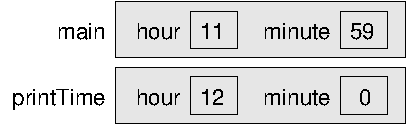
\includegraphics{figs/stack.pdf}

For each method there is a gray box called a {\bf frame} that contains
the method's parameters and variables.  The name of the method
appears outside the frame.  As usual, the value of each variable
is drawn inside a box with the name of the variable beside it.



\section {Methods with multiple parameters}
\label{time}
\index{parameter!multiple}
\index{method!multiple parameter}
\index{class!Time}

The syntax for declaring and invoking methods with multiple
parameters is a common source of errors.  First, remember
that you have to declare the type of every parameter.  For
example

\begin{code}
    public static void printTime(int hour, int minute) {
        System.out.print(hour);
        System.out.print(":");
        System.out.println(minute);
    }
\end{code}
%
It might be tempting to write {\tt int hour, minute}, but
that format is only legal for variable declarations, not
parameter lists.

Another common source of confusion is that you do not have
to declare the types of arguments.  The following is wrong!

\begin{code}
    int hour = 11;
    int minute = 59;
    printTime(int hour, int minute);   // WRONG!
\end{code}
%
In this case, Java can tell the type of {\tt hour}
and {\tt minute} by looking at their declarations.  It is
not necessary to include the type when you pass them
as arguments.  The correct
syntax is {\tt printTime(hour, minute)}.


\section {Methods that return values}
\index{value method}
\index{method!value}

Some of the methods we are using,
like the {\tt Math} methods, return values.  Other methods,
like {\tt println} and {\tt newLine}, perform an action but
they don't return a value.  That raises some questions:

\begin{itemize}

\item What happens if you invoke a method and you don't
do anything with the result (i.e. you don't assign it to
a variable or use it as part of a larger expression)?

\item What happens if you use a {\tt print} method as part
of an expression, like {\tt System.out.println("boo!") + 7}?

\item Can we write methods that return values, or are we
stuck with things like {\tt newLine} and {\tt printTwice}?

\end{itemize}

The answer to the third question is ``yes, you can write methods that
return values,'' and we'll see how in a couple of chapters.  I
leave it up to you to answer the other two questions by trying them
out.  In fact, any time you have a question about what is legal or
illegal in Java, a good way to find out is to ask the compiler.


\section{Glossary}

\begin{description}

\item[initialization:]  A statement that declares a new variable
and assigns a value to it at the same time.
\index{initialization}

\item[floating-point:] A type of variable (or value) that can contain
fractions as well as integers.  The floating-point type we will
use is {\tt double}.

\item[class:]  A named collection of methods.  So far, we have used
the {\tt Math} class and the {\tt System} class, and we have
written classes named {\tt Hello} and {\tt NewLine}.

\item[method:]  A named sequence of statements that performs a
useful function.  Methods may or may not take parameters, and may
or may not return a value.

\item[parameter:]  A piece of information a method requires before
it can run.  Parameters are variables: they contain values and have types.

\item[argument:]  A value that you provide when you invoke a
method.  This value must have the same type as the corresponding
parameter.

\item[frame:] A structure (represented by a gray box in stack diagrams)
that contains a method's parameters and variables.

\item[invoke:]  Cause a method to execute.

\index{floating-point}
\index{class}
\index{method}
\index{parameter}
\index{argument}

\end{description}

\section{Exercises}

\begin{exercise}

Draw a stack frame that shows the state of the program in Section~\ref{time}
when {\tt main} invokes {\tt printTime}
with the arguments {\tt 11} and {\tt 59}.

\end{exercise}

\begin{exercise}

The point of this exercise is to practice reading code and to
make sure that you understand the flow of execution through
a program with multiple methods.

\begin{enumerate}

\item What is the output of the following program?  Be precise
about where there are spaces and where there are newlines.

HINT: Start by describing in words what {\tt ping} and
{\tt baffle} do when they are invoked.

\item Draw a stack diagram that shows the state of the program
the first time {\tt ping} is invoked.

\end{enumerate}

\begin{code}
  public static void zoop() {
    baffle();
    System.out.print("You wugga ");
    baffle();
  }

  public static void main(String[] args) {
    System.out.print("No, I ");
    zoop();
    System.out.print("I ");
    baffle();
  }

  public static void baffle() {
    System.out.print("wug");
    ping();
  }

  public static void ping() {
    System.out.println(".");
  }
\end{code}

\end{exercise}


\begin{exercise}

The point of this exercise is to make sure you understand how
to write and invoke methods that take parameters.

\begin{enumerate}

\item Write the first line of a method named {\tt zool} that
takes three parameters: an {\tt int} and two {\tt Strings}.

\item Write a line of code that invokes {\tt zool}, passing
as arguments the value {\tt 11}, the name of your first pet,
and the name of the street you grew up on.
\end{enumerate}

\end{exercise}


\begin{exercise}

The purpose of this exercise is to take code from a previous exercise
and encapsulate it in a method that takes parameters.  You should
start with a working solution to Exercise~\ref{ex.date}.

\begin{enumerate}

\item Write a method called {\tt printAmerican}
that takes the day, date, month and year as parameters and that
prints them in American format.

\item Test your method by invoking it from {\tt main} and passing
appropriate arguments.  The output should look something like this
(except that the date might be different):
%
\begin{stdout}
Saturday, July 16, 2011
\end{stdout}
%
\item Once you have debugged {\tt printAmerican}, write another
method called {\tt printEuropean} that prints the date in
European format.

\end{enumerate}
\end{exercise}



